% This LaTeX document needs to be compiled with XeLaTeX.
\documentclass[10pt]{article}
\usepackage[utf8]{inputenc}
\usepackage{graphicx}
\usepackage[export]{adjustbox}
\graphicspath{ {./images/} }
\usepackage{amsmath}
\usepackage{amsfonts}
\usepackage{amssymb}
\usepackage[version=4]{mhchem}
\usepackage{stmaryrd}
\usepackage{multirow}
\usepackage[fallback]{xeCJK}
\usepackage{polyglossia}
\usepackage{fontspec}
\setCJKmainfont{Noto Serif CJK TC}

\setmainlanguage{polish}
\setmainfont{CMU Serif}

\title{EGZAMIN MATURALNY Z MATEMATYKI }

\author{}
\date{}


\begin{document}
\maketitle
\begin{center}

\includegraphics[max width=\textwidth]{2024_11_21_99a977d92f90f1d0fb7fg-01(1)}
\end{center}

\section*{Arkusz I \\
 POZIOM PODSTAWOWY}
\section*{ARKUSZ I}
\section*{Czas pracy 120 minut}
\section*{Instrukcja dla zdającego}
\begin{enumerate}
  \item Sprawdź, czy arkusz egzaminacyjny zawiera 14 stron (zadania 1-11). Ewentualny brak zgłoś przewodniczącemu zespołu nadzorującego egzamin.
  \item Rozwiązania zadań i odpowiedzi zamieść w miejscu na to przeznaczonym.
  \item W rozwiązaniach zadań przedstaw tok rozumowania prowadzący do ostatecznego wyniku.
  \item Pisz czytelnie. Używaj długopisu/pióra tylko z czarnym tuszem/atramentem.
  \item Nie używaj korektora, a błędne zapisy przekreśl.
  \item Pamiętaj, że zapisy w brudnopisie nie podlegają ocenie.
  \item Obok każdego zadania podana jest maksymalna liczba punktów, którą możesz uzyskać za jego poprawne rozwiązanie.
  \item Możesz korzystać z zestawu wzorów matematycznych, cyrkla i linijki oraz kalkulatora.
  \item Wypełnij tę część karty odpowiedzi, którą koduje zdający. Nie wpisuj żadnych znaków w części przeznaczonej dla egzaminatora.
  \item Na karcie odpowiedzi wpisz swoją datę urodzenia i PESEL. Zamaluj \(\square\) pola odpowiadajace cyfrom numeru PESEL. Będne zaznaczenie otocz kółkiem i i zaznacz właściwe.
\end{enumerate}

Za rozwiązanie wszystkich zadań można otrzymać łacznie\\
50 punktów

Życzymy powodzenia!

Wypełnia zdający przed rozpoczęciem pracy\\
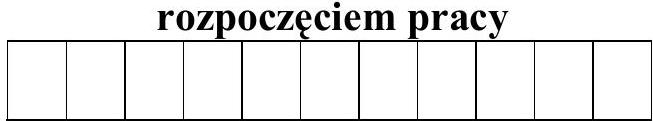
\includegraphics[max width=\textwidth, center]{2024_11_21_99a977d92f90f1d0fb7fg-01}

PESEL ZDAJĄCEGO\\
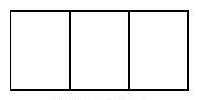
\includegraphics[max width=\textwidth, center]{2024_11_21_99a977d92f90f1d0fb7fg-01(2)}

KOD\\
ZDAJĄCEGO

\section*{Zadanie 1. (3 pkt)}
Dane są zbiory: \(A=\{x \in R:|x-4| \geq 7\}, B=\left\{x \in R: x^{2}>0\right\}\). Zaznacz na osi liczbowej:\\
a) zbiór \(A\),\\
b) zbiór \(B\),\\
c) zbiór \(C=B \backslash A\).\\
a)\\

\includegraphics[max width=\textwidth, center]{2024_11_21_99a977d92f90f1d0fb7fg-02(2)}\\
b)\\

\includegraphics[max width=\textwidth, center]{2024_11_21_99a977d92f90f1d0fb7fg-02(1)}\\
c)\\

\includegraphics[max width=\textwidth, center]{2024_11_21_99a977d92f90f1d0fb7fg-02}

\begin{center}
\begin{tabular}{|c|l|c|c|c|}
\hline
\multirow{2}{*}{\begin{tabular}{c}
Wypetnia \\
egzaminator! \\
\end{tabular}} & Nr czynności & 1.1. & 1.2. & 1.3. \\
\cline { 2 - 5 }
 & Maks. liczba pkt & 1 & 1 & 1 \\
\cline { 2 - 5 }
 & Uzyskana liczba pkt &  &  &  \\
\hline
\end{tabular}
\end{center}

\section*{Zadanie 2. (3 pkt)}
W wycieczce szkolnej bierze udział 16 uczniów, wśród których tylko czworo zna okolicę. Wychowawca chce wybrać w sposób losowy 3 osoby, które mają pójść do sklepu. Oblicz prawdopodobieństwo tego, że wśród wybranych trzech osób będą dokładnie dwie znające okolicę.\\

\includegraphics[max width=\textwidth, center]{2024_11_21_99a977d92f90f1d0fb7fg-03}

\begin{center}
\begin{tabular}{|c|l|c|c|c|}
\hline
\multirow{2}{*}{\begin{tabular}{c}
Wypelnia \\
egzaminator! \\
\end{tabular}} & Nr czynności & 2.1. & 2.2. & 2.3. \\
\cline { 2 - 5 }
 & Maks. liczba pkt & 1 & 1 & 1 \\
\cline { 2 - 5 }
 & Uzyskana liczba pkt &  &  &  \\
\hline
\end{tabular}
\end{center}

\section*{Zadanie 3. (5 pht)}
Kostka masła produkowanego przez pewien zakład mleczarski ma nominalną mase 20 dag. W czasie kontroli zakładu zważono 150 losowo wybranych kostek masła. Wyniki badań przedstawiono w tabeli.

\begin{center}
\begin{tabular}{|l|c|c|c|c|c|c|}
\hline
Masa kostki masła ( w dag ) & 16 & 18 & 19 & 20 & 21 & 22 \\
\hline
Liczba kostek masła & 1 & 15 & 24 & 68 & 26 & 16 \\
\hline
\end{tabular}
\end{center}

a) Na podstawie danych przedstawionych w tabeli oblicz średnią arytmetyczną oraz odchylenie standardowe masy kostki masła.\\
b) Kontrola wypada pozytywnie, jeśli średnia masa kostki masła jest równa masie nominalnej i odchylenie standardowe nie przekracza 1 dag. Czy kontrola zakładu wypadła pozytywnie? Odpowiedź uzasadnij.\\

\includegraphics[max width=\textwidth, center]{2024_11_21_99a977d92f90f1d0fb7fg-04}

\begin{center}
\begin{tabular}{|c|l|c|c|c|}
\hline
\multirow{2}{*}{\begin{tabular}{c}
Wypetnia \\
egzaminator! \\
\end{tabular}} & Nr czynności & 3.1. & 3.2. & 3.3. \\
\cline { 2 - 5 }
 & Maks. liczba pkt & 2 & 2 & 1 \\
\cline { 2 - 5 }
 & Uzyskana liczba pkt &  &  &  \\
\hline
\end{tabular}
\end{center}

\section*{Zadanie 4. (4 pkt)}
Dany jest rosnący ciag geometryczny, w którym \(a_{1}=12, a_{3}=27\).\\
a) Wyznacz iloraz tego ciagu.\\
b) Zapisz wzór, na podstawie którego można obliczyć wyraz \(a_{n}\), dla każdej liczby naturalnej \(n \geq 1\).\\
c) Oblicz wyraz \(a_{6}\).

\begin{center}
\begin{tabular}{|c|c|c|c|c|c|c|c|c|c|c|c|c|c|c|c|c|c|c|c|c|c|}
\hline
 &  &  &  &  &  &  &  &  &  &  &  &  &  &  &  &  &  &  &  &  &  \\
\hline
 &  &  &  &  &  &  &  &  &  &  &  &  &  &  &  &  &  &  &  &  &  \\
\hline
 &  &  &  &  &  &  &  &  &  &  &  &  &  &  &  &  &  &  &  &  &  \\
\hline
 &  &  &  &  &  &  &  &  &  &  &  &  &  &  &  &  &  &  &  &  &  \\
\hline
 &  &  &  &  &  &  &  &  &  &  &  &  &  &  &  &  &  &  &  &  &  \\
\hline
 &  &  &  &  &  &  &  &  &  &  &  &  &  &  &  &  &  &  &  &  &  \\
\hline
 &  &  &  &  &  &  &  &  &  &  &  &  &  &  &  &  &  &  &  &  &  \\
\hline
 &  &  &  &  &  &  &  &  &  &  &  &  &  &  &  &  &  &  &  &  &  \\
\hline
 &  &  &  &  &  &  &  &  &  &  &  &  &  &  &  &  &  &  &  &  &  \\
\hline
 &  &  &  &  &  &  &  &  &  &  &  &  &  &  &  &  &  &  &  &  &  \\
\hline
 &  &  &  &  &  &  &  &  &  &  &  &  &  &  &  &  &  &  &  &  &  \\
\hline
 &  &  &  &  &  &  &  &  &  &  &  &  &  &  &  &  &  &  &  &  &  \\
\hline
 &  &  &  &  &  &  &  &  &  &  &  &  &  &  &  &  &  &  &  &  &  \\
\hline
 &  &  &  &  &  &  &  &  &  &  &  &  &  &  &  &  &  &  &  &  &  \\
\hline
 &  &  &  &  &  &  &  &  &  &  &  &  &  &  &  &  &  &  &  &  &  \\
\hline
 &  &  &  &  &  &  &  &  &  &  &  &  &  &  &  &  &  &  &  &  &  \\
\hline
 &  &  &  &  &  &  &  &  &  &  &  &  &  &  &  &  &  &  &  &  &  \\
\hline
 &  &  &  &  &  &  &  &  &  &  &  &  &  &  &  &  &  &  &  &  &  \\
\hline
 &  &  &  &  &  &  &  &  &  &  &  &  &  &  &  &  &  &  &  &  &  \\
\hline
 &  &  &  &  &  &  &  &  &  &  &  &  &  &  &  &  &  &  &  &  &  \\
\hline
 &  &  &  &  &  &  &  &  &  &  &  &  &  &  &  &  &  &  &  &  &  \\
\hline
 &  &  &  &  &  &  &  &  &  &  &  &  &  &  &  &  &  &  &  &  &  \\
\hline
 &  &  &  &  &  &  &  &  &  &  &  &  &  &  &  &  &  &  &  &  &  \\
\hline
 &  &  &  &  &  &  &  &  &  &  &  &  &  &  &  &  &  &  &  &  &  \\
\hline
 &  &  &  &  &  &  &  &  &  &  &  &  &  &  &  &  &  &  &  &  &  \\
\hline
 &  &  &  &  &  &  &  &  &  &  &  &  &  &  &  &  &  &  &  &  &  \\
\hline
 &  &  &  &  &  &  &  &  &  &  &  &  &  &  &  &  &  &  &  &  &  \\
\hline
 &  &  &  &  &  &  &  &  &  &  &  &  &  &  &  &  &  &  &  &  &  \\
\hline
 &  &  &  &  &  &  &  &  &  &  &  &  &  &  &  &  &  &  &  &  &  \\
\hline
 &  &  &  &  &  &  &  &  &  &  &  &  &  &  &  &  &  &  &  &  &  \\
\hline
 &  &  &  &  &  &  &  &  &  &  &  &  &  &  &  &  &  &  &  &  &  \\
\hline
 &  &  &  &  &  &  &  &  &  &  &  &  &  &  &  &  &  &  &  &  &  \\
\hline
 &  &  &  &  &  &  &  &  &  &  &  &  &  &  &  &  &  &  &  &  &  \\
\hline
 &  &  &  &  &  &  &  &  &  &  &  &  &  &  &  &  &  &  &  &  &  \\
\hline
 &  &  &  &  &  &  &  &  &  &  &  &  &  &  &  &  &  &  &  &  &  \\
\hline
 &  &  &  &  &  &  &  &  &  &  &  &  &  &  &  &  &  &  &  &  &  \\
\hline
 &  &  &  &  &  &  &  &  &  &  &  &  &  &  &  &  &  &  &  &  &  \\
\hline
 &  &  &  &  &  &  &  &  &  &  &  &  &  &  &  &  &  &  &  &  &  \\
\hline
 &  &  &  &  &  &  &  &  &  &  &  &  &  &  &  &  &  &  &  &  &  \\
\hline
 &  &  &  &  &  &  &  &  &  &  &  &  &  &  &  &  &  & 到 &  &  &  \\
\hline
 &  &  &  &  &  &  &  &  &  &  &  &  &  &  &  &  &  &  &  &  &  \\
\hline
\end{tabular}
\end{center}

\begin{center}
\begin{tabular}{|c|l|c|c|c|}
\hline
\multirow{2}{*}{\begin{tabular}{c}
Wypetnia \\
egzaminator! \\
\end{tabular}} & Nr czynności & 4.1. & 4.2. & 4.3. \\
\cline { 2 - 5 }
 & Maks. liczba pkt & 2 & 1 & 1 \\
\cline { 2 - 5 }
 & Uzyskana liczba pkt &  &  &  \\
\hline
\end{tabular}
\end{center}

\section*{Zadanie 5. (3 pkt)}
Wiedząc, że \(0^{\circ} \leq \alpha \leq 360^{\circ}, \sin \alpha<0\) oraz \(4 \operatorname{tg} \alpha=3 \sin ^{2} \alpha+3 \cos ^{2} \alpha\)\\
a) oblicz \(\operatorname{tg} \alpha\),\\
b) zaznacz w układzie współrzędnych kąt \(\alpha\) i podaj współrzędne dowolnego punktu, różnego od początku układu współrzędnych, który leży na końcowym ramieniu tego kąta.\\
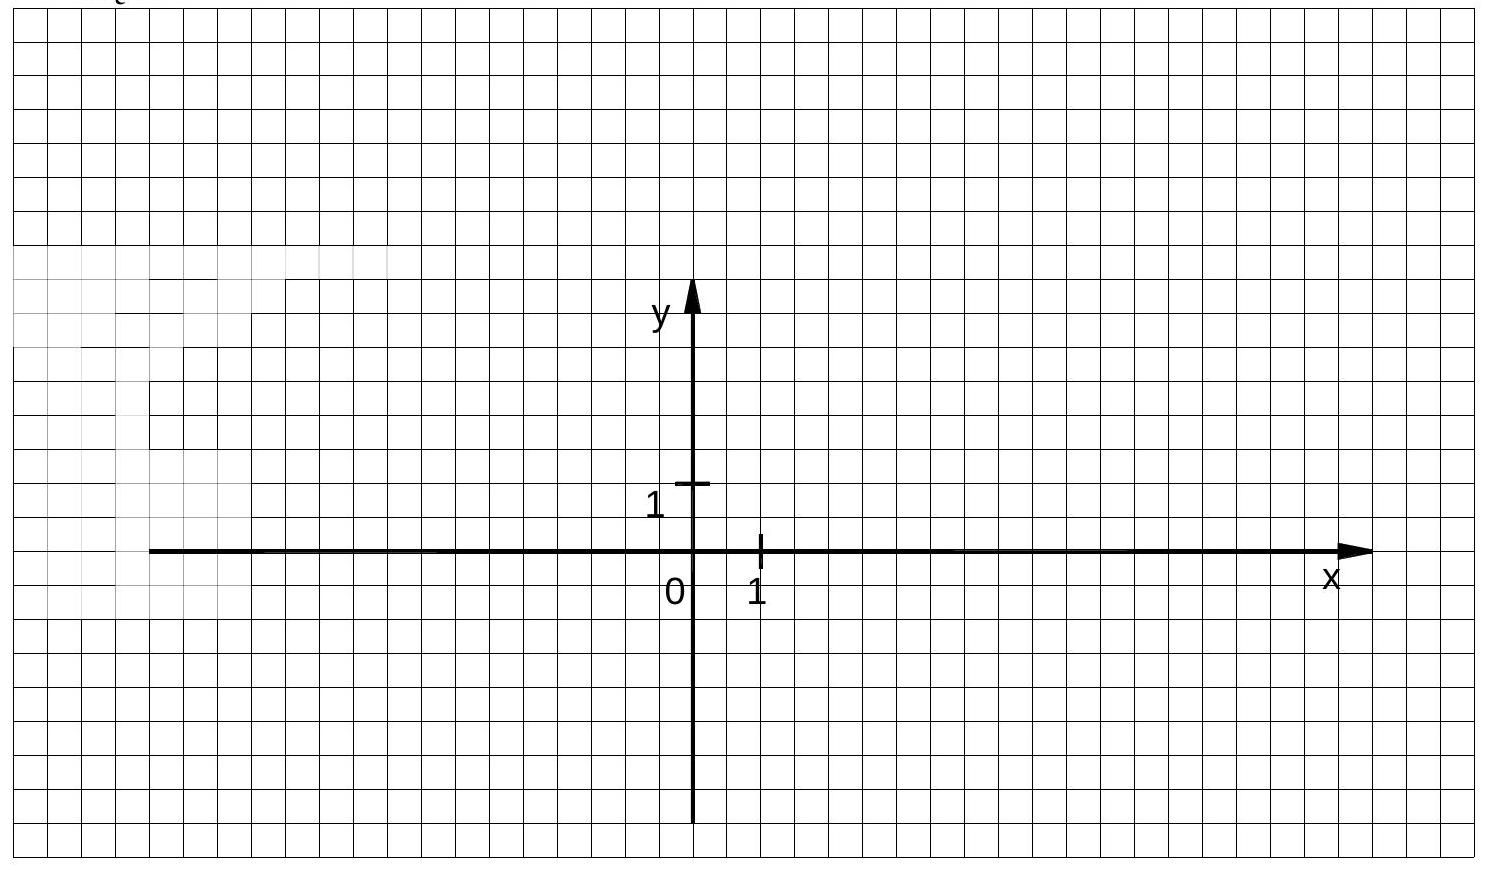
\includegraphics[max width=\textwidth, center]{2024_11_21_99a977d92f90f1d0fb7fg-06}

\begin{center}
\begin{tabular}{|c|c|c|c|c|c|c|c|c|c|c|c|c|c|c|c|c|c|c|c|c|c|}
\hline
 &  &  &  &  &  &  &  &  &  &  & 到 &  &  &  &  &  &  &  &  &  &  \\
\hline
 &  &  &  &  &  &  &  &  &  &  &  &  &  &  &  &  &  &  &  &  &  \\
\hline
 &  &  &  &  &  &  &  &  &  &  &  &  &  &  &  &  &  &  &  &  &  \\
\hline
 &  &  &  &  &  &  &  &  &  &  &  &  &  &  &  &  &  &  &  &  &  \\
\hline
 &  &  &  &  &  &  &  &  &  &  &  &  &  &  &  &  &  &  &  &  &  \\
\hline
 &  &  &  &  &  &  &  &  &  &  &  &  &  &  &  &  &  &  &  &  &  \\
\hline
 &  &  &  &  &  &  &  &  &  &  &  &  &  &  &  &  &  &  &  &  &  \\
\hline
 &  &  &  &  &  &  &  &  &  &  &  &  &  &  &  &  &  &  &  &  &  \\
\hline
 &  &  &  &  &  &  &  &  &  &  &  &  &  &  &  &  &  &  &  &  &  \\
\hline
 &  &  &  &  &  &  &  &  &  &  &  &  &  &  &  &  &  &  &  &  &  \\
\hline
 &  &  &  &  &  &  &  &  &  &  &  &  &  &  &  &  &  &  &  &  &  \\
\hline
 &  &  &  &  &  &  &  &  &  &  &  &  &  &  &  &  &  &  &  &  &  \\
\hline
 &  &  &  &  &  &  &  &  &  &  &  &  &  &  &  &  &  &  &  &  &  \\
\hline
 &  &  &  &  &  &  &  &  &  &  &  &  &  &  &  &  &  &  &  &  &  \\
\hline
 &  &  &  &  &  &  &  &  &  &  &  &  &  &  &  &  &  &  &  &  &  \\
\hline
 &  &  &  &  &  &  &  &  &  &  &  &  &  &  &  &  &  &  &  &  &  \\
\hline
 &  &  &  &  &  &  &  &  &  &  &  &  &  &  &  &  &  &  &  &  &  \\
\hline
 &  &  &  &  &  &  &  &  &  &  &  &  &  &  &  &  &  &  &  &  &  \\
\hline
 &  &  &  &  &  &  &  &  &  &  &  &  &  &  &  &  &  &  &  &  &  \\
\hline
 &  &  &  &  &  &  &  &  &  &  &  &  &  &  &  &  &  &  &  &  &  \\
\hline
 &  &  &  &  &  &  &  &  &  &  &  &  &  &  &  &  &  &  &  &  &  \\
\hline
 &  &  &  &  &  &  &  &  &  &  &  &  &  &  &  &  &  &  &  &  &  \\
\hline
 &  &  &  &  &  &  &  &  &  &  &  &  &  &  &  &  &  &  &  &  &  \\
\hline
 &  &  &  &  &  &  &  &  &  &  &  &  &  &  &  &  &  &  &  &  &  \\
\hline
\end{tabular}
\end{center}

\begin{center}
\begin{tabular}{|c|l|c|c|c|}
\hline
\multirow{2}{*}{\begin{tabular}{c}
Wypetnia \\
egzaminator! \\
\end{tabular}} & Nr czynności & 5.1. & 5.2. & 5.3. \\
\cline { 2 - 5 }
 & Maks. liczba pkt & 1 & 1 & 1 \\
\cline { 2 - 5 }
 & Uzyskana liczba pkt &  &  &  \\
\hline
\end{tabular}
\end{center}

\section*{Zadanie 6. (7 pkt)}
Państwo Nowakowie przeznaczyli 26000 zł na zakup działki. Do jednej z ofert dołączono rysunek dwóch przylegających do siebie działek w skali 1:1000. Jeden metr kwadratowy gruntu w tej ofercie kosztuje 35 zł. Oblicz, czy przeznaczona przez państwa Nowaków kwota wystarczy na zakup działki \(P_{2}\).\\
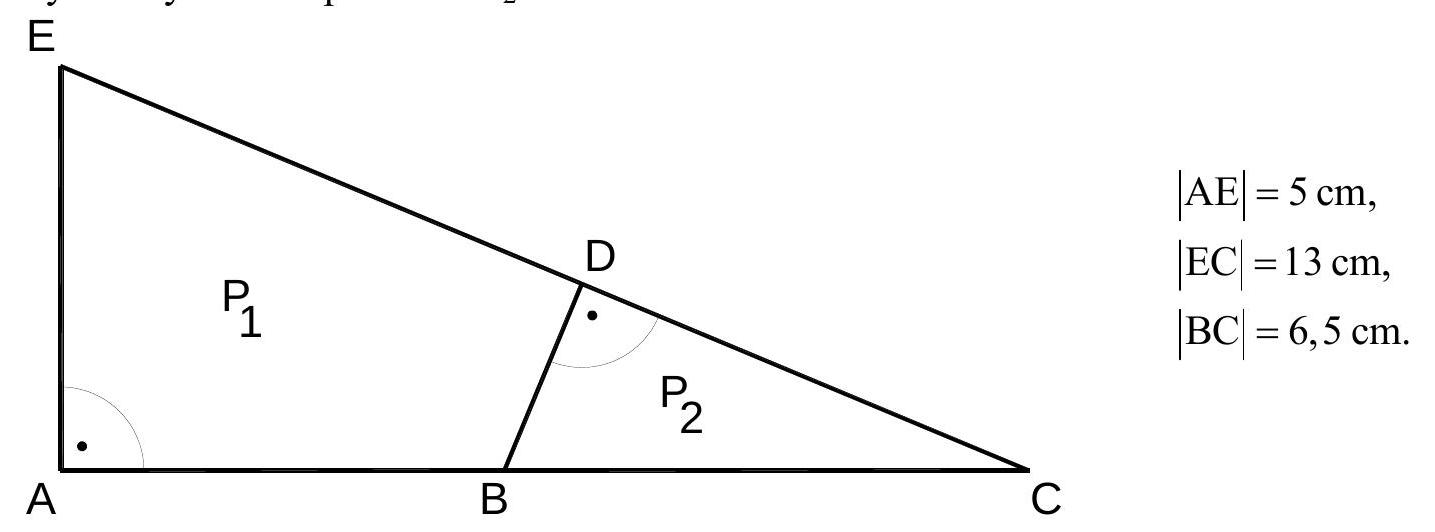
\includegraphics[max width=\textwidth, center]{2024_11_21_99a977d92f90f1d0fb7fg-07}\\

\includegraphics[max width=\textwidth, center]{2024_11_21_99a977d92f90f1d0fb7fg-07(1)}

\begin{center}
\begin{tabular}{|c|l|c|c|c|c|c|c|c|}
\hline
\multirow{2}{*}{\begin{tabular}{c}
Wypelnia \\
egzaminator: \\
\end{tabular}} & Nr czynności & 6.1. & 6.2. & 6.3. & 6.4. & 6.5. & 6.6. & 6.7. \\
\cline { 2 - 9 }
 & Maks. liczba pkt & 1 & 1 & 1 & 1 & 1 & 1 & 1 \\
\cline { 2 - 9 }
 & Uzyskana liczba pkt &  &  &  &  &  &  &  \\
\hline
\end{tabular}
\end{center}

\section*{Zadanie 7. (5 pkt)}
Szkic przedstawia kanał ciepłowniczy, którego przekrój poprzeczny jest prostokątem. Wewnątrz kanału znajduje się rurociąg składający się z trzech rur, każda o średnicy zewnętrznej 1 m . Oblicz wysokość i szerokość kanału ciepłowniczego. Wysokość zaokraglij do \(0,01 \mathrm{~m}\).\\
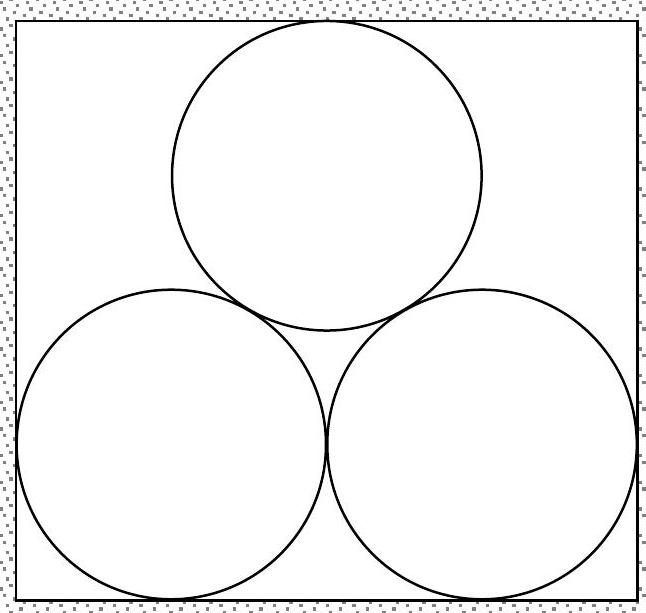
\includegraphics[max width=\textwidth, center]{2024_11_21_99a977d92f90f1d0fb7fg-08}\\

\includegraphics[max width=\textwidth, center]{2024_11_21_99a977d92f90f1d0fb7fg-08(1)}

\begin{center}
\begin{tabular}{|c|l|c|c|c|c|}
\hline
\multirow{2}{*}{\begin{tabular}{c}
Wypetnia \\
egzaminator! \\
\end{tabular}} & Nr czynności & 7.1. & 7.2. & 7.3. & 7.4. \\
\cline { 2 - 6 }
 & Maks. liczba pkt & 1 & 1 & 2 & 1 \\
\hline
 & Uzyskana liczba pkt &  &  &  &  \\
\hline
\end{tabular}
\end{center}

\section*{Zadanie 8. (5 pht)}
Dana jest funkcja \(f(x)=-x^{2}+6 x-5\).\\
a) Naszkicuj wykres funkcji \(f\) i podaj jej zbiór wartości.\\
b) Podaj rozwiązanie nierówności \(f(x) \geq 0\).\\
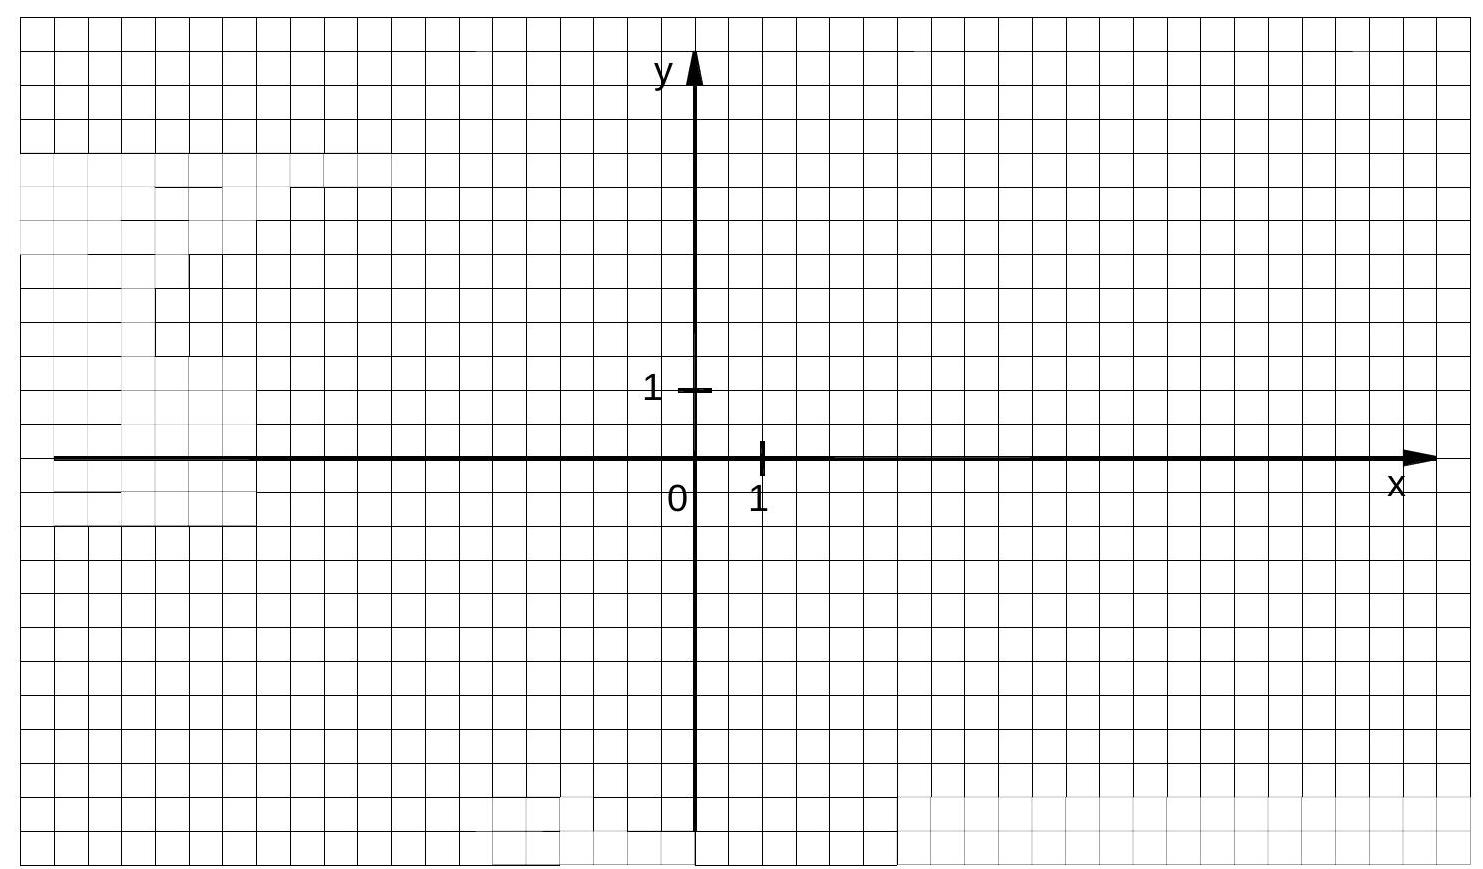
\includegraphics[max width=\textwidth, center]{2024_11_21_99a977d92f90f1d0fb7fg-09}

\begin{center}
\begin{tabular}{|c|c|c|c|c|c|c|c|c|c|c|c|c|c|c|c|c|c|c|c|c|c|c|c|c|c|c|c|c|c|c|}
\hline
 &  &  &  &  &  &  &  &  &  &  &  &  &  &  &  &  &  &  &  &  &  &  &  &  &  &  &  &  &  &  \\
\hline
 &  &  &  &  &  &  &  &  &  &  &  &  &  &  &  &  &  &  &  &  &  &  &  &  &  &  &  &  &  &  \\
\hline
 &  &  &  &  &  &  &  &  &  &  &  &  &  &  &  &  &  &  &  &  &  &  &  &  &  &  &  &  &  &  \\
\hline
 &  &  &  &  &  &  &  &  &  &  &  &  &  &  &  &  &  &  &  &  &  &  &  &  &  &  &  &  &  &  \\
\hline
 &  &  &  &  &  &  &  &  &  &  &  &  &  &  &  &  &  &  &  &  &  &  &  &  &  &  &  &  &  &  \\
\hline
 &  &  &  &  &  &  &  &  &  &  &  &  &  &  &  &  &  &  &  &  &  &  &  &  &  &  &  &  &  &  \\
\hline
 &  &  &  &  &  &  &  &  &  &  &  &  &  &  &  &  &  &  &  &  &  &  &  &  &  &  &  &  &  &  \\
\hline
 &  &  &  &  &  &  &  &  &  &  &  &  &  &  &  &  &  &  &  &  &  &  &  &  &  &  &  &  &  &  \\
\hline
 &  &  &  &  &  &  &  &  &  &  &  &  &  &  &  &  &  &  &  &  &  &  &  &  &  &  &  &  &  &  \\
\hline
 &  &  &  &  &  &  &  &  &  &  &  &  &  &  &  &  &  &  &  &  &  &  &  &  &  &  &  &  &  &  \\
\hline
 &  &  &  &  &  &  &  &  &  &  &  &  &  &  &  &  &  &  &  &  &  &  &  &  &  &  &  &  &  &  \\
\hline
 &  &  &  &  &  &  &  &  &  &  &  &  &  &  &  &  &  &  &  &  &  &  &  &  &  &  &  &  &  &  \\
\hline
 &  &  &  &  &  &  &  &  &  &  &  &  &  &  &  &  &  &  &  &  &  &  &  &  &  &  &  &  &  &  \\
\hline
 &  &  &  &  &  &  &  &  &  &  &  &  &  &  &  &  &  &  &  &  &  &  &  &  &  &  &  &  &  &  \\
\hline
 &  &  &  &  &  &  &  &  &  &  &  &  &  &  &  &  &  &  &  &  &  &  &  &  &  &  &  &  &  &  \\
\hline
 &  &  &  &  &  &  &  &  &  &  &  &  &  &  &  &  &  &  &  &  &  &  &  &  &  &  &  &  &  &  \\
\hline
 &  &  &  &  &  &  &  &  &  &  &  &  &  &  &  &  &  &  &  &  &  &  &  &  &  &  &  &  &  &  \\
\hline
 &  &  &  &  &  &  &  &  &  &  &  &  &  &  &  &  &  &  &  &  &  &  &  &  &  &  &  &  &  &  \\
\hline
 &  &  &  &  &  &  &  &  &  &  &  &  &  &  &  &  &  &  &  &  &  &  &  &  &  &  &  &  &  &  \\
\hline
 &  &  &  &  &  &  &  &  &  &  &  &  &  &  &  &  &  &  &  &  &  &  &  &  &  &  &  &  &  &  \\
\hline
 &  &  &  &  &  &  &  &  &  &  &  &  &  &  &  &  &  &  &  &  &  &  &  &  &  &  &  &  &  &  \\
\hline
 &  &  &  &  &  &  &  &  &  &  &  &  &  &  &  &  &  &  &  &  &  &  &  &  &  &  &  &  &  &  \\
\hline
 &  &  &  &  &  &  &  &  &  &  &  &  &  &  &  &  &  &  &  &  &  &  &  &  &  &  &  &  &  &  \\
\hline
 &  &  &  &  &  &  &  &  &  &  &  &  &  &  &  &  &  &  &  &  &  &  &  &  &  &  &  &  &  &  \\
\hline
 &  &  &  &  &  &  &  &  &  &  &  &  &  &  &  &  &  &  &  &  &  &  &  &  &  &  &  &  &  &  \\
\hline
\end{tabular}
\end{center}

\begin{center}
\begin{tabular}{|c|l|c|c|c|c|c|}
\hline
\multirow{2}{*}{\begin{tabular}{c}
Wypełnia \\
egzaminator! \\
\end{tabular}} & Nr czynności & 8.1. & 8.2. & 8.3. & 8.4. & 8.5. \\
\cline { 2 - 7 }
 & Maks. liczba pkt & 1 & 1 & 1 & 1 & 1 \\
\cline { 2 - 7 }
 & Uzyskana liczba pkt &  &  &  &  &  \\
\hline
\end{tabular}
\end{center}

\section*{Zadanie 9. (6 pkt)}
Dach wieży ma kształt powierzchni bocznej ostrosłupa prawidłowego czworokątnego, którego krawędź podstawy ma długość 4 m . Ściana boczna tego ostrosłupa jest nachylona do płaszczyzny podstawy pod kątem \(60^{\circ}\).\\
a) Sporządź pomocniczy rysunek i zaznacz na nim podane w zadaniu wielkości.\\
b) Oblicz, ile sztuk dachówek należy kupić, aby pokryć ten dach, wiedząc, że do pokrycia \(1 \mathrm{~m}^{2}\) potrzebne są 24 dachówki. Przy zakupie należy doliczyć \(8 \%\) dachówek na zapas.\\

\includegraphics[max width=\textwidth, center]{2024_11_21_99a977d92f90f1d0fb7fg-10}

\begin{center}
\begin{tabular}{|c|l|c|c|c|c|c|}
\hline
\multirow{2}{*}{\begin{tabular}{c}
Wypełnia \\
egzaminator! \\
\end{tabular}} & Nr czynności & 9.1. & 9.2. & 9.3. & 9.4. & 9.5. \\
\cline { 2 - 7 }
 & Maks. liczba pkt & 1 & 1 & 1 & 2 & 1 \\
\cline { 2 - 7 }
 & Uzyskana liczba pkt &  &  &  &  &  \\
\hline
\end{tabular}
\end{center}

\section*{Zadanie 10. (6 pkt)}
Liczby 3 i -1 są pierwiastkami wielomianu \(W(x)=2 x^{3}+a x^{2}+b x+30\).\\
a) Wyznacz wartości współczynników \(a\) i \(b\).\\
b) Oblicz trzeci pierwiastek tego wielomianu.\\

\includegraphics[max width=\textwidth, center]{2024_11_21_99a977d92f90f1d0fb7fg-11}

\begin{center}
\begin{tabular}{|c|l|c|c|c|c|c|c|}
\hline
\multirow{2}{*}{\begin{tabular}{c}
Wypetnia \\
egzaminator! \\
\end{tabular}} & Nr czynności & 10.1. & 10.2. & 10.3. & 10.4. & 10.5. & 10.6. \\
\cline { 2 - 8 }
 & Maks. liczba pkt & 1 & 1 & 1 & 1 & 1 & 1 \\
\cline { 2 - 8 }
 & Uzyskana liczba pkt &  &  &  &  &  &  \\
\hline
\end{tabular}
\end{center}

\section*{Zadanie 11. (3 pkt)}
Sumę \(S=\frac{3}{1 \cdot 4}+\frac{3}{4 \cdot 7}+\frac{3}{7 \cdot 10}+\ldots+\frac{3}{301 \cdot 304}+\frac{3}{304 \cdot 307}\) można obliczyć w następujący sposób:\\
a) sumę \(S\) zapisujemy w postaci

\[
S=\frac{4-1}{4 \cdot 1}+\frac{7-4}{7 \cdot 4}+\frac{10-7}{10 \cdot 7}+\ldots+\frac{304-301}{304 \cdot 301}+\frac{307-304}{307 \cdot 304}
\]

b) każdy składnik tej sumy przedstawiamy jako różnicę ułamków

\[
\begin{gathered}
S=\left(\frac{4}{4 \cdot 1}-\frac{1}{4 \cdot 1}\right)+\left(\frac{7}{7 \cdot 4}-\frac{4}{7 \cdot 4}\right)+\left(\frac{10}{10 \cdot 7}-\frac{7}{10 \cdot 7}\right)+\ldots+\left(\frac{304}{304 \cdot 301}-\frac{301}{304 \cdot 301}\right)+\left(\frac{307}{307 \cdot 304}-\frac{304}{307 \cdot 304}\right) \\
\operatorname{stact} S=\left(1-\frac{1}{4}\right)+\left(\frac{1}{4}-\frac{1}{7}\right)+\left(\frac{1}{7}-\frac{1}{10}\right)+\ldots+\left(\frac{1}{301}-\frac{1}{304}\right)+\left(\frac{1}{304}-\frac{1}{307}\right) \\
\quad \text { więc } S=1-\frac{1}{4}+\frac{1}{4}-\frac{1}{7}+\frac{1}{7}-\frac{1}{10}+\ldots+\frac{1}{301}-\frac{1}{304}+\frac{1}{304}-\frac{1}{307}
\end{gathered}
\]

c) obliczamy sumę, redukując parami wyrazy sąsiednie, poza pierwszym i ostatnim \(S=1-\frac{1}{307}=\frac{306}{307}\).\\
Postępując w analogiczny sposób, oblicz sumę \(S_{1}=\frac{4}{1 \cdot 5}+\frac{4}{5 \cdot 9}+\frac{4}{9 \cdot 13}+\ldots+\frac{4}{281 \cdot 285}\).

\begin{center}
\begin{tabular}{|c|c|c|c|c|c|c|c|c|c|c|c|c|c|c|c|c|c|c|c|c|c|c|c|}
\hline
 &  &  &  &  &  &  &  &  &  &  &  &  &  &  &  &  &  &  &  &  &  &  &  \\
\hline
 &  &  &  &  &  &  &  &  &  &  &  &  &  &  &  &  &  &  &  &  &  &  &  \\
\hline
 &  &  &  &  &  &  &  &  &  &  &  &  &  &  &  &  &  &  &  &  &  &  &  \\
\hline
 &  &  &  &  &  &  &  &  &  &  &  &  &  &  &  &  &  &  &  &  &  &  &  \\
\hline
 &  &  &  &  &  &  &  &  &  &  &  &  &  &  &  &  &  &  &  &  &  &  &  \\
\hline
 &  &  &  &  &  &  &  &  &  &  &  &  &  &  &  &  &  &  &  &  &  &  &  \\
\hline
 &  &  &  &  &  &  &  &  &  &  &  &  &  &  &  &  &  &  &  &  &  &  &  \\
\hline
 &  &  &  &  &  &  &  &  &  &  &  &  &  &  &  &  &  &  &  &  &  &  &  \\
\hline
 &  &  &  &  &  &  &  &  &  &  &  &  &  &  &  &  &  &  &  &  &  &  &  \\
\hline
 &  &  &  &  &  &  &  &  &  &  &  &  &  &  &  &  &  &  &  &  &  &  &  \\
\hline
 &  &  &  &  &  &  &  &  &  &  &  &  &  &  &  &  &  &  &  &  &  &  &  \\
\hline
 &  &  &  &  &  &  &  &  &  &  &  &  &  &  &  &  &  &  &  &  &  &  &  \\
\hline
 &  &  &  &  &  &  &  &  &  &  &  &  &  &  &  &  &  &  &  &  &  &  &  \\
\hline
 &  &  &  &  &  &  &  &  &  &  &  &  &  &  &  &  &  &  &  &  &  &  &  \\
\hline
 &  &  &  &  &  &  &  &  &  &  &  &  &  &  &  &  &  &  &  &  &  &  &  \\
\hline
 &  &  &  &  &  &  &  &  &  &  &  &  &  &  &  &  &  &  &  &  &  &  &  \\
\hline
 &  &  &  &  &  &  &  &  &  &  &  &  &  &  &  &  &  &  &  &  &  &  &  \\
\hline
 &  &  &  &  &  &  &  &  &  &  &  &  &  &  &  &  &  &  &  &  &  &  &  \\
\hline
 &  &  &  &  &  &  &  &  &  &  &  &  &  &  &  &  &  &  &  &  &  &  &  \\
\hline
 &  &  &  &  &  &  &  &  &  &  &  &  &  &  &  &  &  &  &  &  &  &  &  \\
\hline
 &  &  &  &  &  &  &  &  &  &  &  &  &  &  &  &  &  &  &  &  &  &  &  \\
\hline
 &  &  &  &  &  &  &  &  &  &  &  &  &  &  &  &  &  &  &  &  &  &  &  \\
\hline
 &  &  &  &  &  &  &  &  &  &  &  &  &  &  &  &  &  &  &  &  &  &  &  \\
\hline
 &  &  &  &  &  &  &  &  &  &  &  &  &  &  &  &  &  &  &  &  &  &  &  \\
\hline
 &  &  &  &  &  &  &  &  &  &  &  &  &  &  &  &  &  &  &  &  &  &  &  \\
\hline
 &  &  &  &  &  &  &  &  &  &  &  &  &  &  &  &  &  &  &  &  &  &  &  \\
\hline
 &  &  &  &  &  &  &  &  &  &  &  &  &  &  &  &  &  &  &  &  &  &  &  \\
\hline
 &  &  &  &  &  &  &  &  &  &  &  &  &  &  &  &  &  &  &  &  &  &  &  \\
\hline
 &  &  &  &  &  &  &  &  &  &  &  &  &  &  &  &  &  &  &  &  &  &  &  \\
\hline
 &  &  &  &  &  &  &  &  &  &  &  &  &  &  &  &  &  &  &  &  &  &  &  \\
\hline
 &  &  &  &  &  &  &  &  &  &  &  &  &  &  &  &  &  &  &  &  &  &  &  \\
\hline
 &  &  &  &  &  &  &  &  &  &  &  &  &  &  &  &  &  &  &  &  &  &  &  \\
\hline
\end{tabular}
\end{center}

\begin{center}

\includegraphics[max width=\textwidth]{2024_11_21_99a977d92f90f1d0fb7fg-13}
\end{center}

\begin{center}
\begin{tabular}{|c|l|c|c|c|}
\hline
\multirow{2}{*}{\begin{tabular}{c}
Wypelnia \\
egzaminator! \\
\end{tabular}} & Nr czynności & 11.1. & 11.2. & 11.3. \\
\cline { 2 - 5 }
 & Maks. liczba pkt & 1 & 1 & 1 \\
\cline { 2 - 5 }
 & Uzyskana liczba pkt &  &  &  \\
\hline
\end{tabular}
\end{center}

\section*{BRUDNOPIS}

\end{document}